\section{Introduction}\label{sec:intro}

Nowadays, the CAE analysis is often performed at an earlier stage in the digital product development process, in order to validate various design alternatives quickly. In such cases, the models are simplified not only for quicker and fairly accurate results, but also to save on precious computing resources and time. Such simplifications involve mainly two phases - first, ``de-featuring'', which deals with suppression of irrelevant features and second, ``idealization'' in which shapes such as slender bar or thin-walled portions are represented by their lower dimensional equivalents (\cite{Dabke1994}) . This paper focuses on one such idealization called ``Midsurface'', typically used for thin-walled models such as sheet metal and plastic parts \cite{FEMBook2009} .  
\todo[backgroundcolor=yellow]{\textbf{Reviewer}: This parameter is important since it is the only place where the authors refer to a quantity that can characterize the
morphology of the domain to be idealized \\ \textbf{Author}: Removed the specifics with hard-coded values and made a general statement}
Midsurface can be envisaged of as a surface, which lies midway of a thin-walled model, mimicking its shape.  It is primarily used to place 2D shell elements in the CAE analysis, which give comparable results vis-a-vis  expensive and slower 3D solid element analysis. Due to this crucial advantage, midsurface functionality is made available  in many commercial CAD-CAE packages. Despite of its criticality, the existing approaches fail to compute a well-connected midsurface, automatically, especially in case of complex models (\cite{Robinson2006},\cite{Automex},\cite{Woo2013},\cite{Stolt2006a},\cite{Lockett2008}). Typical failures are, missing midsurface patches, gaps, overlaps, not lying midway, not mimicking the input shape, etc. Correcting these errors is mostly a manual, tedious and highly time-consuming process, requiring from several hours to days. This correction time can be nearly equivalent to the time it can take to create the midsurface manually from scratch (\cite{Stolt2006}).  So, an automated and robust computation method is a critical need of the hour.

One of the major impediments in the development of the algorithm for automatic computation of the midsurface, is the lack of its precise definition (\cite{Ramanathan2004}).  Expectations vary, making it hard to develop a formal logic (Figure ~\ref{fig:step}). As seen in Figure \ref{fig_stfl}, one may want a gradual change between the two midsurface patches at the site of a step, whereas, others may choose to either mimic (Figure ~\ref{fig_stmk}) or ignore the step (if within certain limit) and just follow the bigger face (Figure ~\ref{fig_sts}) or just two separate patches representing two different thicknesses  (Figure ~\ref{fig_spr}). Automatic methods need to be able to customize for such variations.


\bigskip

\def \myfigstepcolumnwidth{0.16}

\begin{figure}[h!]
\centering     %%% not \center
\subfloat[Model]{\label{fig_stmodel}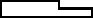
\includegraphics[width=\myfigstepcolumnwidth\linewidth]{../Common/images/Step_part.pdf}} \quad
\subfloat[Gradual at step]{\label{fig_stfl}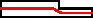
\includegraphics[width=\myfigstepcolumnwidth\linewidth]{../Common/images/Step_follows.pdf}}  \quad
\subfloat[Mimicking step]{\label{fig_stmk}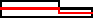
\includegraphics[width=\myfigstepcolumnwidth\linewidth]{../Common/images/Step_mimic.pdf}}   \quad
\subfloat[Ignoring step]{\label{fig_sts}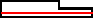
\includegraphics[width=\myfigstepcolumnwidth\linewidth]{../Common/images/Step_straight.pdf}}  \quad
\subfloat[Disjoint at step]{\label{fig_spr}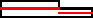
\includegraphics[width=\myfigstepcolumnwidth\linewidth]{../Common/images/Step_separate.pdf}}
\caption{Expectations vary with regards to desired Midsurface}
\label{fig:step}
\end{figure}


\bigskip

\todo[backgroundcolor=yellow]{\textbf{Reviewer}: The authors mention the multiple expectations regarding the definition of mid­surfaces. Indeed, the authors look for a purely geometric definition of mid­surfaces whereas the idealization process is a mechanical process, i.e. it involves both mechanics and geometry. This aspect should be put forward rather than reducing the mid­surface computation to geometric transformations only. Otherwise, it means that the authors restrict themselves to a subset of configurations where their proposed approach can be applied. In this context, the proposed approach does not bring new contribution compared to the work of Armstrong et al. or Boussuge et al., for example.\\\textbf{Author}: Clearly mentioned that its a CAD algorithm and does not take CAE aspects into consideration. Even within CAD domain, there are quite a few deficiencies in the works of Armstrong or Boussuge that this paper tries to address}

Applications can also dictate the shape of the midsurface desired. CAE considerations, such as symmetry, change the midsurface (say, an axisymmetric part may analyze only one sector and not the whole part). To bring definitiveness in this work, CAE considerations are not taken into account. The reason being, the midsurface can have potential applications other than CAE as well, such as feature recognition, shape retrieval/transmission, etc. Application-specific aspects can also be potentially integrated into the current work, but this has been currently kept out of scope of this work/paper. The goal of this work is to compute a midsurface that geometrically and topologically represents/mimics the input shape.


\section{Related work}

Some of the prominent methods for computing midsurface (generically called ``medial'') are thinning, Chordal Axis Transform (CAT), parametric, Medial Axis Transform (MAT), Midsurface Abstraction (MA), etc. (\cite{Lam1992}, \cite{Yogesh2010}). Out of these, MAT and  MA are two of the most researched medial computation techniques (\cite{Sheen2010}). 

\begin{figure}[h!]
\centering     %%% not \center
\subfloat[Model]{\label{fig_tmodel}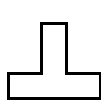
\includegraphics[width=0.23\linewidth]{../Common/images/T_part.pdf}}
\subfloat[MAT]{\label{fig_tmat}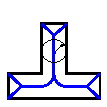
\includegraphics[width=0.23\linewidth]{../Common/images/T_mat.pdf}} \quad
\subfloat[MA]{\label{fig_tma}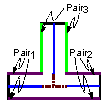
\includegraphics[width=0.23\linewidth]{../Common/images/T_ma.pdf}} \quad
\caption{Midsurface Computation Methods: MAT and MA}
\end{figure}

 MAT is a locus of the center of an inscribed disc of maximal diameter as it rolls around the object's interior (Figure~\ref{fig_tmat}). It was initiated by Blum (\cite{Harry1967}) and  was later developed further into different variations (\cite{Lam1992},\cite{Donaghy1996}, \cite{Attali1997}, \cite{DonaghyArmstrongPrice2000}, \cite{Ramanathan2004}, \cite{Robinson2006}). % RMOVED AS WE WANT LIT SURVEY TO BE JUST ONE PAGE %%Midcurve (Figure~\ref{fig_midcurve}) is a variation of MAT  (Figure~\ref{fig_tmat2}), where it follows the input shape completely and is obtained by processing  (Figure~\ref{fig_process}) extra branches (\cite{Ramanathan2004}).
%\begin{figure}[h!]
%\centering     %%% not \center
%\subfloat[MAT]{\label{fig_tmat2}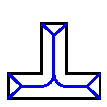
\includegraphics[width=0.3\linewidth]{../Common/images/T_mat2.pdf}}
%\subfloat[Processing]{\label{fig_process}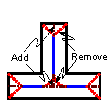
\includegraphics[width=0.3\linewidth]{../Common/images/T_mat_process.pdf}}
%\subfloat[Midcurve]{\label{fig_midcurve}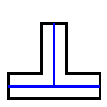
\includegraphics[width=0.3\linewidth]{../Common/images/T_midcurve.pdf}}
%\caption{Processing of MAT}
%\end{figure}
In MA  (Figure~\ref{fig_tma}), opposite faces are detected by ray casting to form face pairs.  Each face-pair computes its own  midsurface patch. Such patches are then ``sewed'' after extending and trimming, wherever necessary. Rezayat (\cite{Rezayat1996}) initiated this approach and it was developed further into various techniques (\cite{Fischer1997},\cite{Elber1999},\cite{Chong2004},\cite{ Hamdi2005},\cite{Sheen2005},\cite{Stolt2006a},\cite{Lee2007},\cite{Cao2009},\cite{Sheen2010},\cite{Woo2013}, \cite{Boussuge2013a}).

Both MAT and MA have quite a few drawbacks. The major ones for MAT are that it creates unnecessary branches and its shape is smaller than the input shape. MA, although more popular amongst the two in the commercial CAD-CAE arena, has two critical challenges, especially in the cases of complex models: detection of the face pairs and resolving interactions amongst the midsurface-patches. For non-trivial cases, there can  be multiple faces in front of each other, with varying degrees of overlaps, different thicknesses, etc., making it difficult to form correct face pairs, giving rise to wrong or missing midsurface patches. If the interaction between the face pairs is not formulated properly, then the appropriate extensions, trimming and joining of their corresponding midsurface patches does not happen properly as well, resulting in gaps, extra untrimmed surfaces, etc.  This paper proposes to address both the problems by proposing an approach leveraging feature information, simplification, abstraction and cellular decomposition as explained in the following sections.

\todo[backgroundcolor=yellow]{\textbf{Reviewer}: The literature review is rather brief and further literature is presented later in the paper. It would be better if this could all be combined together into a single literature section. Present all of the literature review in one section at the beginning of the paper (including the literature in section 2.4). \\ \textbf{Author}: Moved review of cellular methods here.}

%The concept of features, their modeling are surveyed by Shah and Mantyala \cite{Shah1995}. State-of-the-art medial technologies can be found in \cite{Lam1992, Yogesh2010}, whereas simplification is reviewed comprehensively by Thakur et al \cite{Thakur2009}. 

\subsection{Comparative Analysis of the Relevant works}
 Quite a few attempts to compute the midsurface using cellular decomposition are found in the literature \cite{Chong2004},\cite{Cao2009},\cite{Cao2011},\cite{Woo2013}. Table \ref{tab:litsurvey} shows how existing methods  appear limited in terms of geometries and the types of connections  handled, compared to the approach presented here.
\todo[backgroundcolor=yellow]{\textbf{Reviewer}: The authors refer to the heuristics of prior work but the authors don't state precisely the limitations of these heuristics.\\ \textbf{Author}: Explained  pairing was done by CHONG, how BOUSSUGE does only parallel faces, only orthogonal connections etc.  Showed how our approach is more generic}
 
\begin{table}[!htb]
\scriptsize
  \centering 
\resizebox{0.9\linewidth}{!}{ 
\begin{tabular}[htp]{@{} p{0.1\linewidth} p{0.2\linewidth}  p{0.2\linewidth} p{0.2\linewidth} p{0.2\linewidth}@{}}
\toprule
\textbf{Researchers}  &	\textbf{Method} &	 \textbf{Shortcomings}  &	 \textbf{Our Approach}\\ \midrule
\textbf{Chong et al.} \cite{Chong2004}  & 
Concave edge decomposition. Midcurves by collapsing edge pairs. If they form a loop, it creates a midsurface patch. & 
Hard-coded inequalities/values to detect edge-pairs. Connection logic is not generic and comprehensive. &
A generic treatment for the computation of midcurves, midsurface patches and their connections.
\\ \midrule

\textbf{Cao et al.} \cite{Cao2009},\cite{Cao2011} &
Concave edge decomposition. Midsurface patches using face pairs. &  No elaboration on joining method is provided. &  Abstraction is used to avoid face pair problems. Generic logic for joining patches. \\ \midrule

\textbf{Woo} \cite{Woo2013}  &
Maximal volume decomposition \cite{Woo2002}, \cite{Woo2003}.  Midsurface patches using face pairs.  Joins them using union boolean.&
 Criteria for removing unwanted patches does not cater to all situations. Extensions cases not elaborated. Only analytical surfaces and parallel face pairs. &
 Extension and removal of patches using a generic logic.  Caters to variable thickness, non-planar shapes. \\ \midrule


 \textbf{Boussuge et al.} \cite{Boussuge2014}  & 
 Generative decomposition. Recognizes Extrudes of each sub-volume. Creates midsurface patches in each sub-volume and connects them together. &

 
No fillets/chamfers. Only Additive features. Only Extrudes with Analytical surfaces. Expensive MAT to detect thin profiles. Works only on Parallel and Orthogonal connections. &
In-built removal of irrelevant fillet/chamfers. Negative features acceptable. Generic Loft.  Simple rules for morphology detection. Generic logic for any numbers/types of connections.
\\ \midrule

 \textbf{Zhu et al.} \cite{Zhu2015} &
 Virtual Decomposition. Midsurface patches using face pairs. &
  Only 3 connection types. Sampling for mid-points may lose some geometries. &  
   Generic logic for midsurface patch creation as well as their  connections. \\ \bottomrule
\end{tabular}
}
 \caption{Comparison with some relevant Cellular Decomposition-based Midsurface Methods}
  \label{tab:litsurvey}
\end{table}





% Following is the analysis of some of the the relevant works and their points of departures compared to our approach.
%
%\todo[backgroundcolor=yellow]{\textbf{Reviewer}:  Clarify the explanation of the overall method by explaining more clearly how the research presented in this
%paper builds on previous research (your own and that of others). It is important that the reader can
%understand the whole method without reference to the literature. At present the paper is rather confusing in
%structure with the problem, potential solutions and the method all mixed together. Clarify the similarities and
%differences to existing "Divide and Conquer" approach approaches e.g \cite{Woo2013}. There is a lack of arguments and details to evaluate some parts of the
%proposed approach. \\ \textbf{Author}: Clearly mentioned points of departure, superiority, in Literature Survey portion}
%
%\begin{itemize}[noitemsep,topsep=2pt,parsep=2pt,partopsep=2pt]
%\item \textbf{Chong et al.} \cite{Chong2004} : Solids are decomposed at concave edges,  builds midsurface patches in the sub-domains and stitches them together. Medians/midcurves are computed by collapsing edge pairs. Medians, if form a loop, creates a midsurface patch. Shortcomings of this approach are: hard-coded inequalities/values used to detect edge-pairs, connection logic is not generic and comprehensive. In comparison, our approach proposes a generic treatment for the computation of midcurves, midsurface patches and their connections.
%\item \textbf{Cao et al.} \cite{Cao2009,Cao2011}:  Decomposes solids with the help of concave edges and associated face-pairs. Each sub-volume builds midsurface patch using its face pair, but no elaboration on joining method is provided. Overall, the approach presented appears limited both in terms of shapes it could handle as well as extendibility.
%\item \textbf{Woo} \cite{Woo2013} : Decomposes solids using maximal volume method , builds midsurface patches by face-pairing each maximal volume and joins them using union boolean. The criteria given for removing unwanted patches appears incomplete (does not cater to all situations). Also, situations where extensions are needed, are not elaborated.  It works only for analytical surfaces and parallel face pairs. Our work overcomes both the limitations and presents a generic approach for various underlying geometries.
%\item \textbf{Boussuge et al.} \cite{Boussuge2013,Boussuge2013a, Boussuge2014} : Uses generative decomposition to create sub-volumes of Extrude type, creates midsurface patches in each and connects them together with interface-interaction logic. Limitation are:
%\begin{itemize}[noitemsep,topsep=2pt,parsep=2pt,partopsep=2pt]
%\item Decomposition assumes lack of fillets and chamfers in the input model. Our work, without putting any such restriction,  defeatures the input model first, with a set of rules to get the  gross shape.
%\item Works only on the Additive sub-volumes making it difficult to have cuts/holes in midsurface. %Our approach puts forth novel idea of Dormant features to pierce back negative volumes into midsurface.
%\item Recognizes only Extrude features limiting the shapes it can handle. Our approach works on generic Loft feature and is easily extend-able to more generic Loft feature as well.
%\item Uses expensive MAT for morphological assessments to detect idealize-able profiles of sub-volumes. Our work detects the same by simple rules of relative size of Loft profile/guide and graph-topology.
%\item Works only on Parallel and Orthogonal connections, where as our work has no such restriction. It is a generic logic for wider geometry types as well as any numbers/types (topological) of connections.
%\end{itemize}
%\item \textbf{Zhu et al.} \cite{Zhu2015}: Decomposes solids virtually (i.e. no real decomposition but just addition of some topological entities at partitions). Uses face pair for midsurface patches. Only a couple of connection types are supported (`Cross'' is not dealt with). Virtual decomposition does not appear to be applicable and effective in complex cases liked mixed thickness. In comparison, the approach presented here is agnostic to the actual feature-cell-volume shapes as long as they can be modelled as generic Loft type.
%\end{itemize}

\todo[backgroundcolor=yellow]{\textbf{Reviewer}:  When the authors refer to the various algorithms for FBCD, they mix up several approaches: as mentioned earlier, the
work of Boussuge et al. differs from the proposed approach and other references like [29]. Here, the
proposed implementation seems merely equivalent to \cite{BidarraKrakerBronsvoort1998}]. \\ \textbf{Author}: Stated the differences with each. Bidarra does not mention how CD was done, its explained by Woo, My approach works at each feature step and not at final fbd model, making it more local than gobal+maximal like Woo}

\todo[backgroundcolor= yellow]{Reviewer:  what are the advantages of the proposed method over the existing methods? Especially over the reference \cite{Woo2013} \\ \textbf{Author}:  Added}

\subsection{Motivation}
After analyzing various past approaches it can be concluded that, there has been a limited success in computing a well-connected midsurface. Figure \ref{fig_comm} shows output of automatic midsurfacing by two of the leading CAD/CAE commercial applications. English alphabets are chosen as benchmarking examples as they are easy to understand and represent wide variety of shapes and connection types found in the real-life thin-walled parts.

\begin{figure}[h!]
\centering     %%% not \center
\subfloat[Model]{\label{fig_mmodel}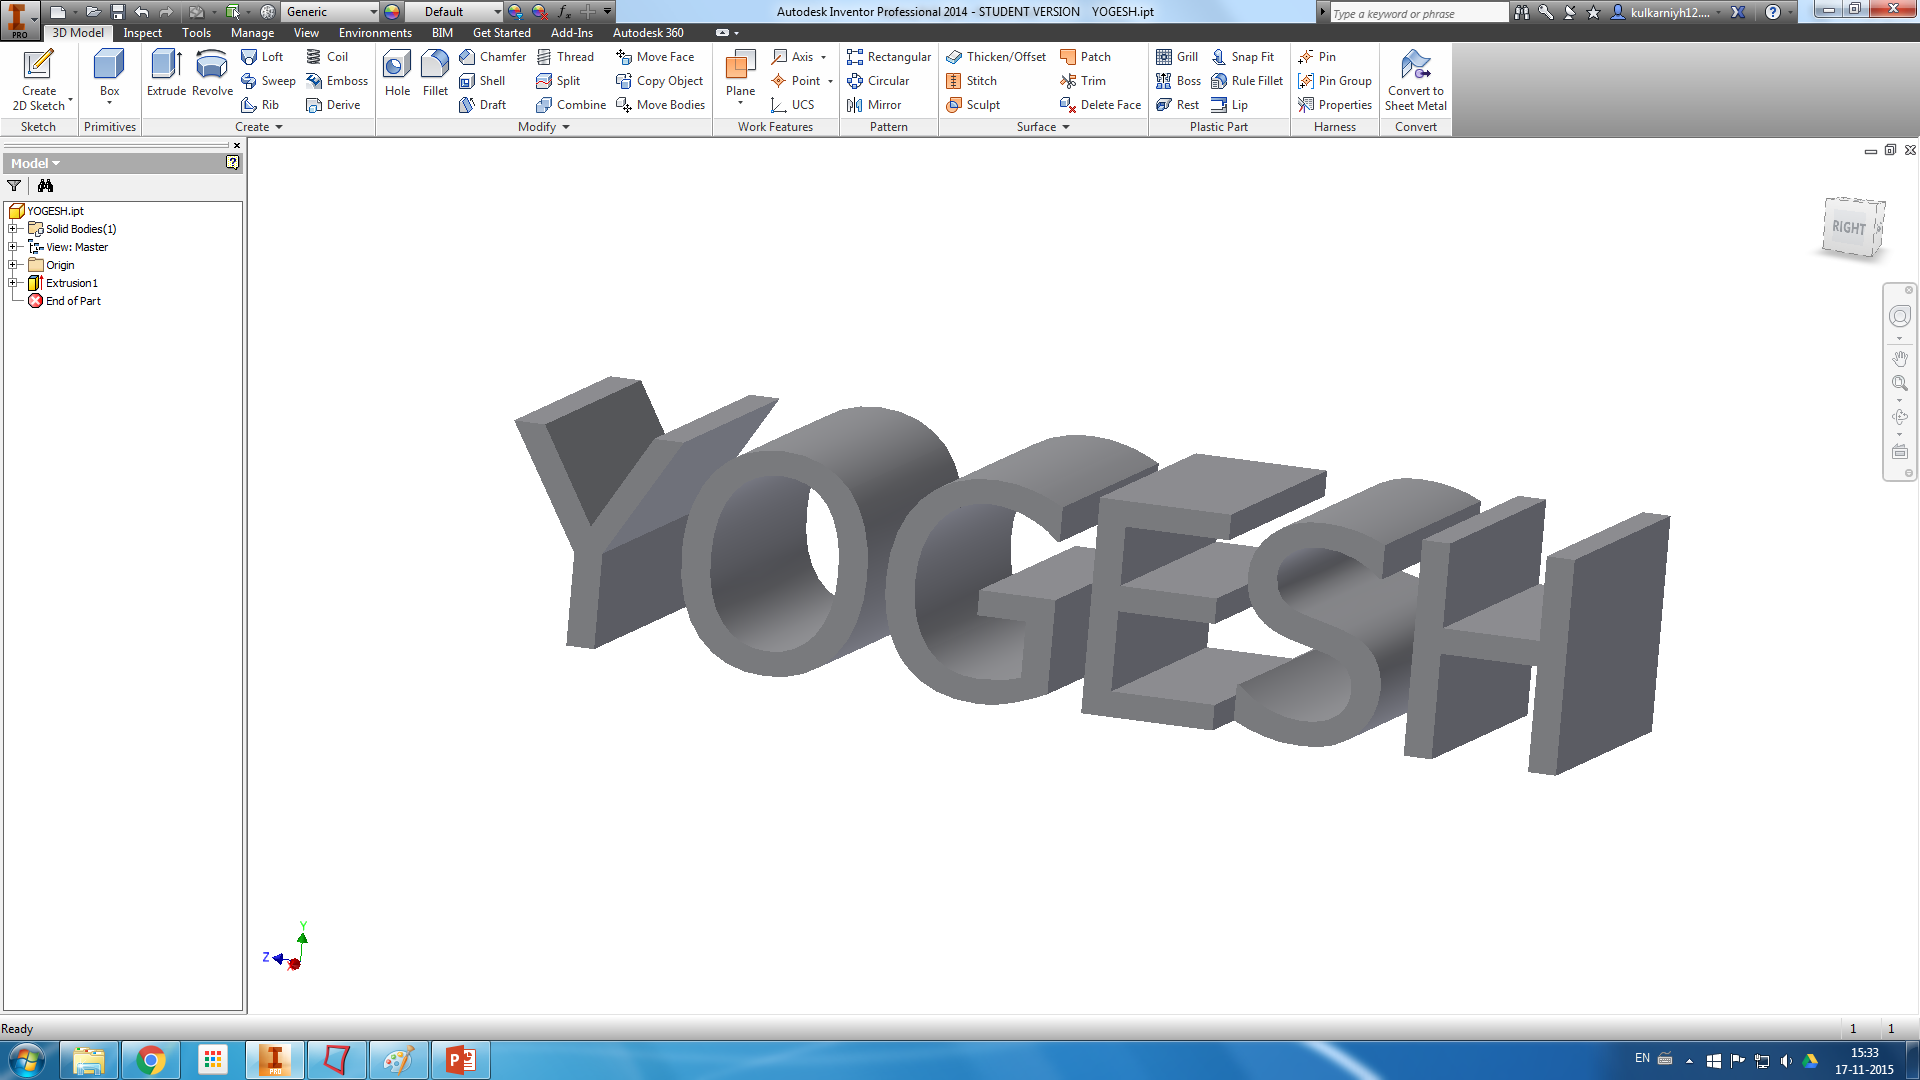
\includegraphics[width=0.3\linewidth]{../Common/images/Yogesh_Inv}} \quad
\subfloat[Midsurface by Application 1]{\label{fig_mcad}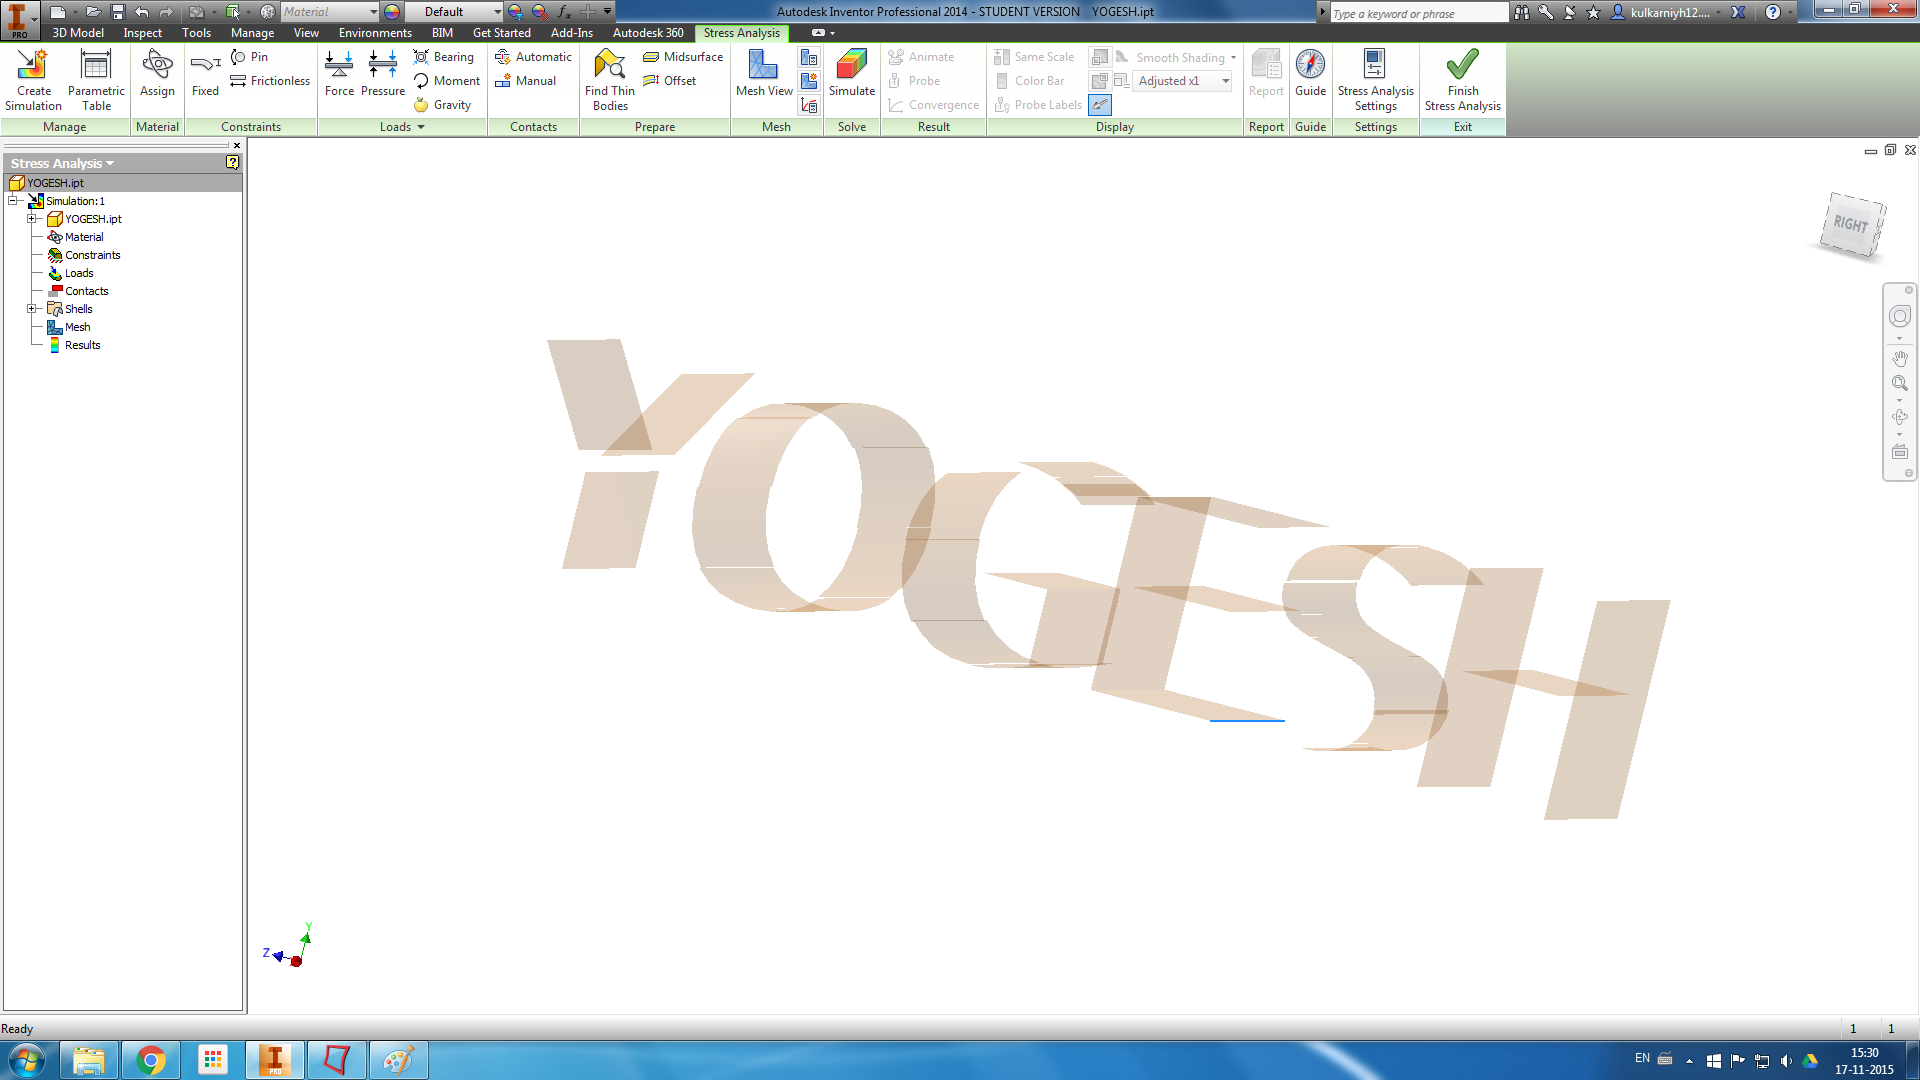
\includegraphics[width=0.3\linewidth]{../Common/images/Yogesh_InvMids}} \quad
\subfloat[Midsurface by Application 2]{\label{fig_mcae}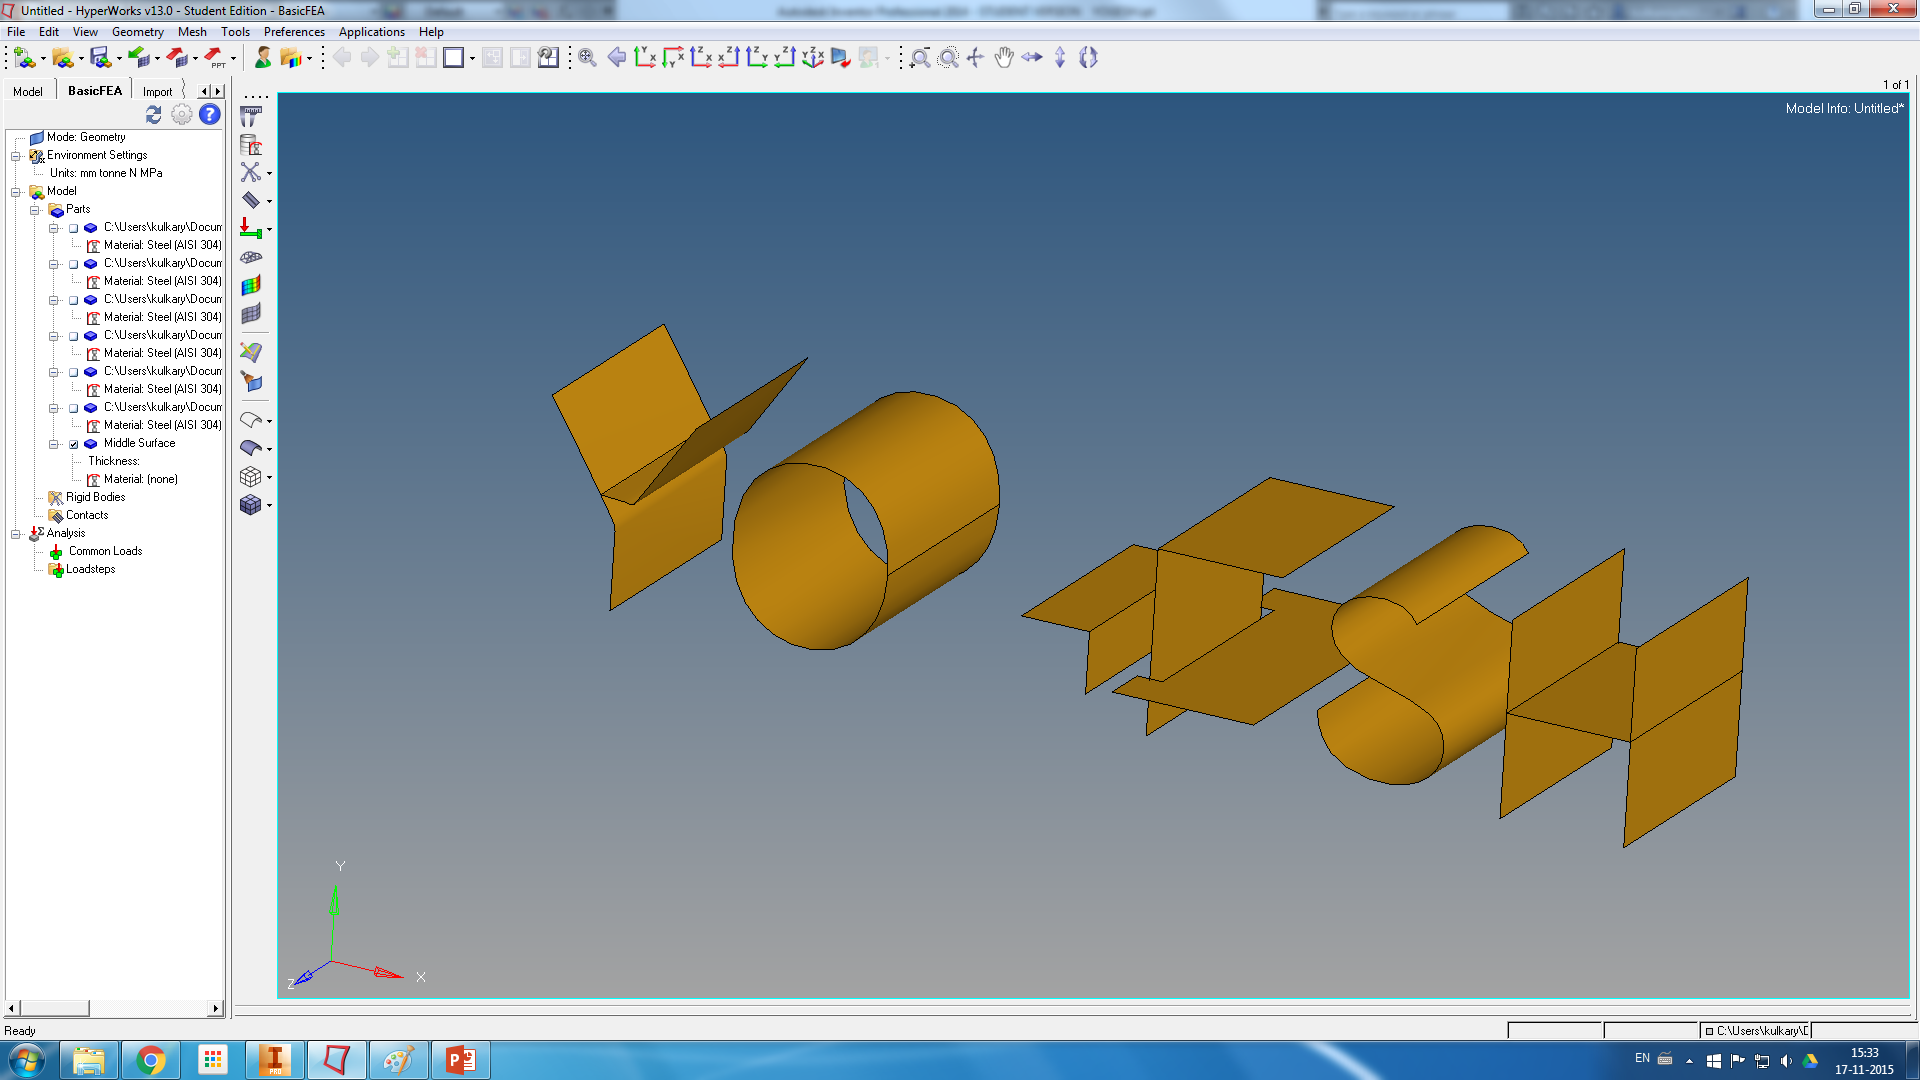
\includegraphics[width=0.3\linewidth]{../Common/images/Yogesh_HM_notOK}} 
\caption{Midsurface outputs of commercial applications}
  \label{fig_comm}
\end{figure}

Midsurface failures such as missing surfaces, gaps, not lying mid-way, etc. can be clearly seen in both the outputs (Figure \ref{fig_mcad},\ref{fig_mcae}). By far, the most widely and commercially used approach appears to be of Midsurface Abstraction (Face Pairing), but, as seen before, even that also is not without any problems. Two of the most critical problems are as follows:

\todo[backgroundcolor=yellow]{\textbf{Reviewer}: On P4 clarify that this paper follows the MA type approach.\\ \textbf{Author}: Wrong understanding of the reviewer. No change.}
	
\subsubsection{Face Pairs Detection Problem}  \label{sec:facepairdetection}
Face pairs, in a way, decompose the whole model into sub-volumes. Each sub-volume creates its own midsurface patch which, later, are ``sewed'' together. In the feature-based CAD model, at each feature step, a tool-body/sub-volume is created and booleaned to the existing model.  Instead of detecting face pairs in the final solid,  feature information, at each step, can be leveraged to compute the midsurface patch for it's corresponding sub-volume.    Here, due to the large number of feature types, writing midsurface-computation for all the feature types separately becomes a tedious task. This work solves this problem by abstracting/generalizing these individual features types into a generic form and then compute midsurface patches for just the generic type. Feature abstraction called ``ABEL'' (\cite{YogeshIITG2014})  has been proposed to generalize the form features into a generic ``Loft'' feature having profile(s) and a guide curve. Midsurface patch can then be computed by sweeping midcurve of the profile(s) along the guide curve (Section \ref{sec:scell}). %%%%%%%% ADD (\cite{YogeshIITG2014}) LATER

\todo[backgroundcolor=yellow]{\textbf{Reviewer}: In section 2 it might be better to keep the solutions separate from the problem.  For example in section 2.1
you refer to the face­pair problem quite clearly but then start to introduce the ABEL approach.  But  this is
then more fully explained later in section 2.4 It might be better to introduce the problems first then leave the
introduction of ABEL to a later section. \\ \textbf{Author}: Moved problems here and not in the Proposed Approach}

\subsubsection{Face-Pair Interaction Problem} \label{sec:facepairinteraction}

In traditional approaches, many midsurface patches fail to get joined, resulting into gaps, overlaps, etc. Midsurface patches need to be connected in the same manner as the face-pairs in the input model are interacted/connected \footnote{Although diagrams used to explain are simplistic/schematic with rectangles depicting feature volumes and lines depicting midsurfaces; in practice these can be of any general shape.} . As there is no theoretical framework encompassing all the possible interaction types, providing a unified logic has not been possible  (\cite{Stolt2006}). Developing connection logic for each of these types separately can be a tedious task. 

\bigskip

\begin{minipage}[c]{\linewidth}
    \begin{minipage}[c]{0.63\linewidth}
 Figure \ref{fig_featinter}  shows representative interaction amongst two sub-volumes along with their own midsurface patches. Sub-volumes $f_1$ and $f_2$ include $m_1$ and $m_2$ as their respective midsurface patches. These can interact in multiple ways, such as, `L', `T', `X', Overlap, Align, etc.
Table \ref{tab:midsinteract} shows how such interactions are dealt with, in the traditional approaches\cite{Rezayat1996}, \cite{Woo2014}, \cite{Boussuge2013}, \cite{Boussuge2013a} using extend/trim so as to connect two midsurface patches. 
    \end{minipage}
    \hfill
    \begin{minipage}[c]{0.37\linewidth}
	\centering 
	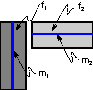
\includegraphics[width=0.65\linewidth]{../Common/images/FeatureInteraction_nonAbel.pdf}
	\captionof{figure}{Feature Interaction. }
	\label{fig_featinter}
    \end{minipage}

\end{minipage}    

\bigskip


\todo[backgroundcolor=yellow]{\textbf{Reviewer}: In section 2.2 clarify how junction types are classified ­ the figures in table 1 are quite confusing. \\ \textbf{Author}: Junctions table changed}

\todo[inline,backgroundcolor=yellow]{\textbf{Reviewer}: There is no justification about the completeness of this list. Indeed, the L type is described incorporating a patch trimming process without justification whereas the authors could consider the abstraction process as mechanical and justify the trimming process. The X type is rather unclear because is refers to a configuration where features cross each other whereas the authors keep on stating that their decomposition into sweeps produces primitives that do not inter penetrate each other. Either this contradicts
the definition of the X type or it means that the X type is effectively unclear. The align case is a particular configuration, that is more restrictive than that proposed in Boussuge et al. and
the overlap configuration is proposed with an additional patch joining the two mid­surfaces. There is no justification for this proposal and it does not mean that the additional patch conforms to the morphological criterion stated in the introduction. This choice is also more restrictive than the configurations processed in Boussuge et al. This is highlighting a lack of consistency of the proposed approach no new contribution compared to prior work. \\ \textbf{Author}: Added more clarification that this table is not part of the proposal but elaborates problems with the existing work.}


\begin{table}[!htb]%[!h]
\centering

\resizebox{\linewidth}{!}{
\begin{tabular}[h]{@{}p{0.12\linewidth} p{0.3\linewidth}  p{0.3\linewidth}  p{0.3\linewidth} @{}} \toprule
{\bf Type} & {\bf Interaction}  & {\bf Midsurface} & {\bf Joining Rule} \\ \midrule  
L / End  &
\adjustbox{valign=t}{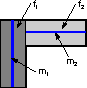
\includegraphics[width=0.8\linewidth]{../Common/images/L_interaction_part.pdf}}  &  
\adjustbox{valign=t}{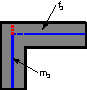
\includegraphics[width=0.8\linewidth]{../Common/images/L_interaction_midsurf.pdf}} &  
New midsurface needs to be extended to meet the existing midsurface. Extra patches of the existing midsurface are trimmed and removed. 
\\ \\ \midrule

T / Middle  &
\adjustbox{valign=t}{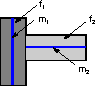
\includegraphics[width=0.9\linewidth]{../Common/images/T_interaction_part.pdf}}  &  
\adjustbox{valign=t}{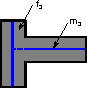
\includegraphics[width=0.8\linewidth]{../Common/images/T_interaction_midsurf.pdf}} &  
New midsurface  needs to be extended to meet the existing midsurface. No trimming is needed.
\\ \\ \midrule

X / Cross &
\adjustbox{valign=t}{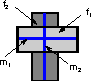
\includegraphics[width=\linewidth]{../Common/images/X_interaction_part.pdf}}  &  
\adjustbox{valign=t}{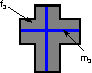
\includegraphics[width=\linewidth]{../Common/images/X_interaction_midsurf.pdf}} &  
New midsurface does not need to be extended. No patch from the existing midsurface is removed. 
\\ \\ \midrule

Align  &
\adjustbox{valign=t}{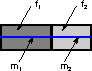
\includegraphics[width=0.9\linewidth]{../Common/images/Align_interaction_part.pdf}}  &  
\adjustbox{valign=t}{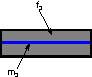
\includegraphics[width=0.9\linewidth]{../Common/images/Align_interaction_midsurf.pdf}} &  
 No adjustment needed.	
\\ \midrule

Overlap  &
\adjustbox{valign=t}{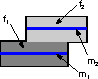
\includegraphics[width=0.9\linewidth]{../Common/images/Overlap_interaction_part.pdf}}  &  
\adjustbox{valign=t}{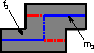
\includegraphics[width=0.9\linewidth]{../Common/images/Overlap_interaction_midsurf.pdf}} &  
 The extra patches are removed from both, the new as well as existing midsurface. New edges are joined with an additional patch.
\\
\bottomrule
\end{tabular}
}
\caption{Interaction of features and their respective midsurface patches}
\label{tab:midsinteract}
\end{table}


It is desirable to provide a consistent-generic method that can be applicable to a wide variety of the cases. Therefore a feature-based cellular decomposition (FBCD) method is employed.  It is a cellular decomposition in the context of features. Bidarra et al. \cite{Bidarra1993}, \cite{Bidarra1997}, \cite{BidarraKrakerBronsvoort1998} showed that feature-based cellular model is a far better/richer representation than the usual feature-based CAD model. They employed it for representing multi-view product geometry, feature operations, etc. Chen et al. presented a unified feature modeling scheme using cellular topology \cite{Chen2006}. Our research, while borrowing this notion of cells with owner features, goes a step further and assigns an abstracted owner-feature, there by making it easier to write a generic algorithm.  In addition, the FBCD used here, as compared to other approaches, is performed, not on the final solid, but in the context of the feature tree, incrementally at each feature step. Thus, the decomposition region remains local, minimizing generation of redundant cells. So, there is no need to utilize the maximal (\cite{Woo2002}) volume strategies to merge a large number of cells computed during the global splittings. 

The proposed approach presented here demonstrates how the given problems are addressed to computed a well-connected midsurface. Table \ref{tbl_fbcmalpha} in the results section \ref{results} shows how the midsurface failures seen in exiting commercial applications have been addressed successfully.

